\chapter{Literature Review} \label{ch1:lit-review}

\section{Deep Learning History}

According to Goodfellow et al., the history of neural network research can be divided into three eras: cybernetics, connectionism, and deep learning~\cite{Goodfellow-et-al-2016}. In the following sections, we adopt this organizational structure to explore the development of deep learning.

\begin{figure}
    \centering
    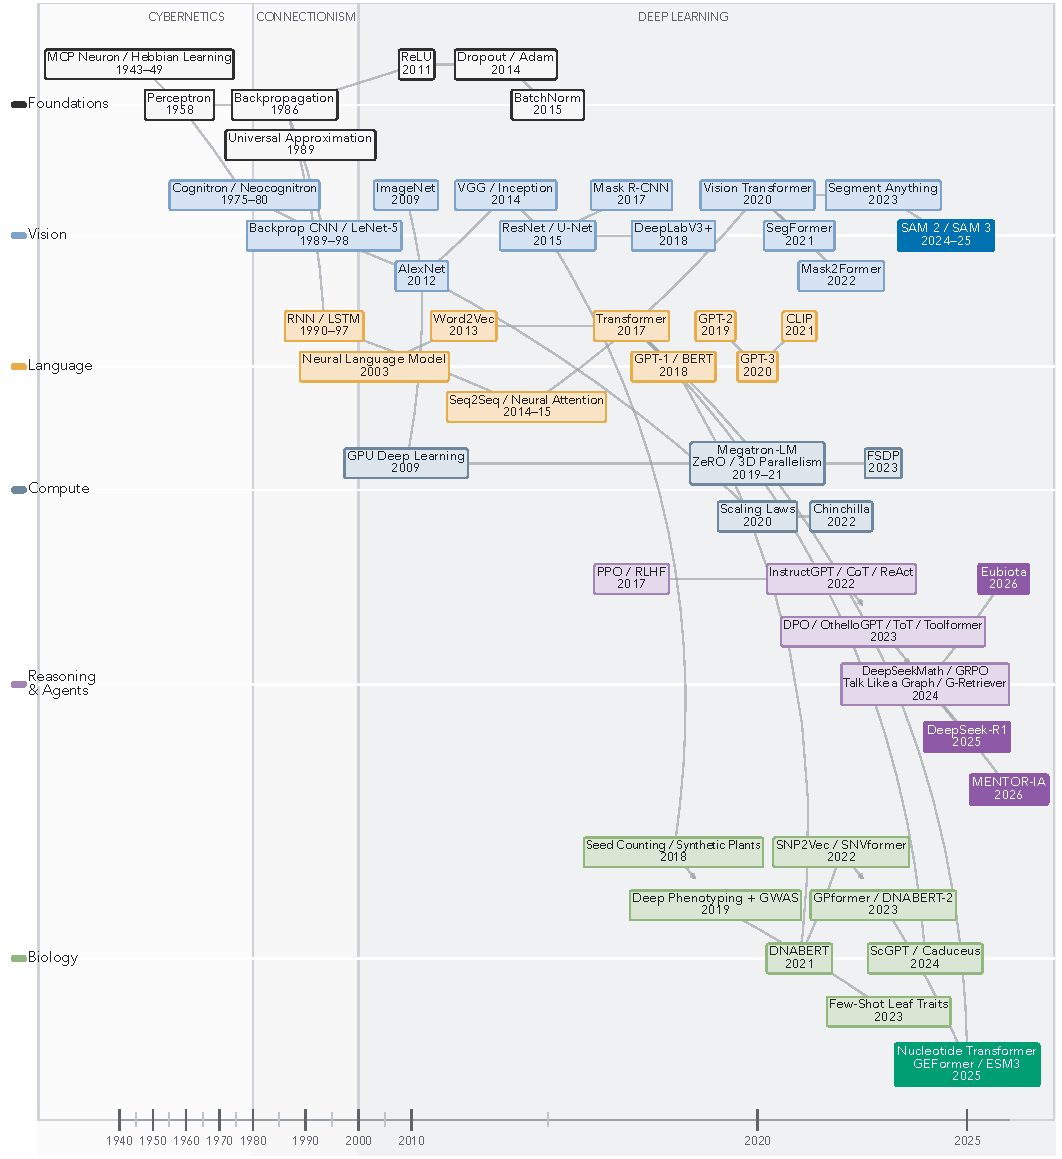
\includegraphics[width=\linewidth]{figures/lit-review/dl-timeline.pdf}
    \caption{History of Deep Learning (1940-2026)}
    \label{fig:ch1-dl-timeline}
\end{figure}


\subsection{Cybernetics}\label{sec:ch1-cybernetics}
The cybernetics era, spanning the 1940s and 1960s, was characterized by early efforts to formalize neural computation through the mathematical modeling of biological nervous systems. The first foundational contribution from this period was presented by McCulloch and Pitts in \textit{A Logical Calculus of Ideas Immanent in Nervous Activity}~\cite{mcculloch1943logical}. The authors provided a modeling framework for neuronal activity through the lens of formal logic; each neuron was framed as a binary computational unit within a larger symbolic logic network. Neuronal activation was determined by inputs corresponding to excitation and inhibition; an output was produced when the aggregated inputs exceeded a fixed threshold. Neurons emitted discrete logical outputs $True$ or $False$, enabling the construction of networks that implemented logical functions. Through this connected framework, McCulloch and Pitts aimed to model neural circuitry in the brain. Importantly, they emphasized that these networks worked over discrete time steps \textit{t}, allowing them to represent sequential dynamics and foreshadowing later concepts like recurrence and memory in neural systems.

Despite establishing a foundational framework for neural computation, the McCulloch-Pitts model exhibited several fundamental limitations. Most notably, the formulation lacked a learning mechanism: network structure and parameters were fixed, requiring manual design rather than learning from data. This static framework stood in contrast to Donald Hebb's work on synaptic plasticity, which postulated that neural pathways are strengthened by repeated co-activation~\cite{hebb1949organization}. Without such a mechanism, the behavior of the McCulloch-Pitts networks could not be modified in response to novel stimuli, limiting this framework's utility for modeling adaptive biological or cognitive processes. 

Furthermore, relying on a purely logical formulation imposed strict representational constraints. Neurons were restricted to binary activation states, resulting in rigid decision boundaries and precluding the learning of continuous representations. Together, these limitations prevented the McCulloch-Pitts networks from scaling to tasks requiring robust function approximation and learning from noisy, high-dimensional data.

The limitations of the McCulloch-Pitts neuron motivated subsequent efforts to develop neural models capable of adaptation, most notably Frank Rosenblatt's 1958 work \textit{The Perceptron: A Probabilistic Model for Information Storage and Organization in the Brain}~\cite{rosenblatt1958perceptron}. Rosenblatt described the perceptron as ``a hypothetical nervous system,'' reflecting an effort to maintain biological inspiration while introducing mechanisms for experience-driven learning. In contrast to the symbolic logic-based formulation of McCulloch and Pitts, Rosenblatt adopted a probabilistic perspective. He argued that the extensive assumptions and structure imposed by their model limited its ability to yield meaningful biological insight. Instead, the perceptron implemented a paradigm that treated data as statistically separable, with a learning mechanism that allowed connections to be reinforced or discouraged via positive or negative stimuli from the data.

While innovations introduced by the perceptron, such as trainable neurons and learning from data, are central to modern deep learning models, the original model had significant shortcomings. Most notably, Rosenblatt's formulation was incapable of representing non-linearly separable functions, with the XOR problem serving as a canonical example. This limitation was a consequence of the perceptron's reliance on linear decision boundaries and its restriction to single-layer architectures, and it severely limited its expressivity. Additionally, Rosenblatt's training rules could not be extended to multi-layer networks due to the lack of a credit assignment mechanism across multiple layers of computation. Combined with the use of binary outputs, these constraints severely limited the functions and representations that could be learned. 

These limitations were rigorously analyzed by Minsky and Papert in their 1969 book \textit{Perceptrons}, whose formal results played a significant role in altering public perception of AI research and contributed to a temporary decline in funding.

%% ADD FIGURE SHOWING THE XOR PROBLEM

\subsection{Connectionism}\label{sec:ch1-connectionism}
Although Minsky and Papert's work provided a rigorous exploration of the limitations of single-layer perceptrons, their critique did not explore whether such constraints could be overcome by multi-layer networks equipped with a credit assignment mechanism. The subsequent era of neural network research, commonly referred to as \textit{connectionism}, was defined by the efforts to address this challenge through the development of multi-layer architectures and the backpropagation algorithm. During this period neural networks also transitioned from primarily symbolic and biologically motivated abstractions toward increasingly general-purpose learning systems. As learning algorithms became more complex and models increased in scale, research increasingly began to favor mathematical tractability over biological interpretability~\cite{rumelhart1986learning, Goodfellow-et-al-2016}.

In 1986, Rumelhart, Hinton, and Williams published \textit{Learning Representations by Back-Propagating Errors}~\cite{rumelhart1986learning}, demonstrating that multi-layer neural networks could be effectively trained through a general solution to the credit assignment problem. Although the mathematical foundations for efficiently computing gradients, known as reverse-mode automatic differentiation, had been previously derived by Seppo Linnainmaa~\cite{linnainmaa1970representation} and applied to neural networks by Paul Werbos~\cite{werbos2005applications}, Rumelhart, Hinton, and Williams popularized the method within the AI community.

The backpropagation algorithm is a gradient-based learning procedure that propagates error information from the network's output backward through successive layers, incrementally modifying each parameter. Using networks trained with backpropagation, the authors showed that non-linearly separable functions could be learned by multilayer networks without relying on hand-designed learning rules.

Backpropagation relies on the differentiability of both the loss function and the network's activation functions, which allow gradients with respect to all parameters to be computed efficiently via the chain rule. This formulation enabled learning signals to be propagated to all network layers, in contrast to earlier approaches like the perceptron, which required a manually specified learning procedure. The formulation of weight updates as an optimization problem allowed neural network training to be extended to more complex multilayer architectures. In addition to backpropagation, this work made several other contributions, such as an explicit learning rate, momentum-based updates, and gradient accumulation, all of which are core to modern neural network optimization.

Beyond their algorithmic contribution, Rumelhart, Hinton, and Williams provided a conceptual framework for understanding multilayer networks. They characterized networks as self-organizing systems that were capable of learning internal representations from data, positing that hidden units in multilayer networks encode features of increasing complexity as network depth increases. These concepts formed the basis of future work in representation learning and motivated the exploration of deeper network architectures to model more complex structures in data.

The representational capabilities of neural networks were mathematically substantiated in 1989, when Cybenko and Hornik et al. independently published proofs of the Universal Approximation Theorem. These works demonstrated that a feed-forward network with a single hidden layer and a finite number of neurons can approximate any continuous function on a compact set~\cite{hornik1989multilayer, cybenko1989approximation}. While Cybenko's work was restricted to networks utilizing sigmoidal activation functions, Hornik et al. extended this result, proving that universality holds for any bounded, non-constant, and monotonically increasing activation function. This work provided a definitive rebuttal to Minsky and Papert's critique of perceptrons~\cite{minsky69perceptrons}, confirming that the limitations they identified were specific to single-layer architectures.

Despite these contributions, connectionist-era neural networks exhibited several limitations relative to modern deep learning models. Most notably, training was restricted by computational resources available at the time, which limited model size and large-scale experimentation. Neural networks were trained on general-purpose central processing units (CPUs), making it impractical to explore deeper architectures or large datasets.

In addition to computational constraints, optimization challenges further limited the effectiveness of early multilayer networks. The authors noted that the backpropagation algorithm could fail in the presence of local minima. With too small a learning rate, weight updates are not enough to traverse the loss landscape toward the global minimum. Furthermore, due to the use of activations such as sigmoid and tanh, gradients could become saturated during backpropagation. Excessively large or small values would fall near the asymptote of these functions, leading to vanishingly small values. As such, the resulting gradients would be small, multiplicatively reducing the learning signal in successive layers. These limitations prevented networks from increasing in depth and learning more complex representations, prompting the development of new methods to overcome these challenges.

\subsection{Deep Learning}\label{sec:ch1-deeplearning}
The transition from connectionism to deep learning emerged from convergent improvements in data, hardware, and algorithms during the late 1990s and early 2000s. These innovations addressed fundamental challenges of the connectionist era, such as vanishing gradients, computational bottlenecks, and convergence failures. Consequently, training networks with more layers became feasible and effective, leading to the era of deep learning, a term popularized by Geoffrey Hinton in 2006~\cite{hinton2006fast}. The pursuit of depth was built on the theoretical foundations laid by Rumelhart, Hinton, and Williams, who demonstrated that hidden layers allow networks to learn more complex hierarchical representations.~\cite{rumelhart1986learning, lecun2015deep}.

A key innovation in the deep learning era was the shift from CPUs to Graphics Processing Units (GPUs). The physical architecture of the GPU is well-suited for homogeneous, parallelizable, and batched operations, specifically massive matrix multiplications central to neural network training. In 2009, Raina et al. published \textit{Large-Scale Deep Unsupervised Learning Using Graphics Processors}, in which they trained Deep Belief Networks (DBNs)~\cite{hinton2006fast} and sparse coding networks~\cite{olshausen1996emergence} using GPUs~\cite{raina2009large}. By storing parameters in the GPU's global memory, parallelizing homogeneous thread operations in stream processors, and using efficient scheduling to reduce overhead times, the authors were able to achieve up to a 72x speedup in DBN training and a 15x speedup in sparse coding training. This acceleration rendered previously intractable problems computationally feasible; the reduction in training time enabled the exploration of deeper architectures and larger datasets, expanding the frontier of neural network training.

In order to fully leverage the benefits of GPU acceleration for neural network training, large, annotated datasets were necessary to avoid overfitting and improve generalization. The earliest advances in dataset construction occurred in the image domain; in the early 2000s, the MNIST dataset of handwritten digits~\cite{lecun1998gradient} served as the benchmark for neural network training. However, this dataset comprised only 10 image classes within a narrow domain, meaning that models trained on this data failed to capture general image recognition capabilities. To overcome these limitations, datasets such as Caltech101~\cite{fei2004learning}, PASCAL VOC~\cite{everingham2010pascal}, and MSRC~\cite{shotton2006textonboost} were developed, providing a wider variety of images and classes for training general-purpose computer vision models. Despite containing more subject diversity than MNIST, these datasets were still relatively small and lacked intra-class variability, with images often being standardized and lacking occlusions, translations, and other perturbations. In 2009, a breakthrough was made with the development and release of the ImageNet dataset~\cite{deng2009imagenet}. The authors of ImageNet leveraged the increasing amount of data available on search engines and the advent of crowdsourcing platforms like Amazon Mechanical Turk to produce a dataset of 3.2 million annotated images following the hierarchical structure of WordNet~\cite{fellbaum1998wordnet}. The availability of large-scale datasets such as ImageNet encouraged the development of neural networks with more layers to capture increasingly abstract and general image representations. This paradigm shift was further catalyzed by the ImageNet Large Scale Visual Recognition Challenge (ILSVRC)~\cite{ILSVRC15}, which will be discussed further in Section~\ref{sec:ch1-imagenet}.

As hardware capabilities improved and massive datasets became available, several algorithmic innovations enabled researchers to train deeper, larger-scale models. One notable breakthrough was the rectified linear unit, or ReLU, which supplanted the sigmoid and hyperbolic tangent (tanh) activation functions that were previously standard~\cite{rumelhart1986learning, lecun1991efficient}. Although ReLU was first utilized in Fukushima's \textit{Cognitron} and \textit{Neocognitron} architectures~\cite{fukushima1975cognitron, fukushima1980neocognitron}, it became widely adopted only after Glorot et al. published \textit{Deep Sparse Rectifier Networks} in 2011~\cite{glorot2011deep}. Glorot et al. showed that ReLU was not only more biologically plausible than its counterparts but also empirically outperformed them in both computer vision and sentiment analysis, especially with deep architectures. ReLU activation enforced network sparsity by setting negative activations to zero and mitigated the vanishing gradient problem with strictly linear positive activations, preventing gradient saturation. 

To fully leverage these properties, weight initialization techniques became widely adopted in deep networks. Building on the work of Glorot and Bengio, who introduced `Xavier initialization' to control the activation variance in sigmoidal networks~\cite{glorot2010understanding}, He et al. introduced `He initialization' to account for the rectification nonlinearity of ReLU~\cite{he2015delving}. These innovations facilitated the training of significantly deeper networks, cementing ReLU as a foundational component of the deep learning era.

To address the generalization challenges posed by these high-capacity models, Srivastava et al. introduced dropout in 2014~\cite{srivastava2014dropout}. Although large datasets such as ImageNet were becoming available, many domains lacked access to millions of labeled training examples. Consequently, deep networks tended to overfit smaller datasets, fitting noise and exhibiting high variance. Dropout ameliorated this issue by regularizing the co-adaptations between neurons. Biologically inspired by sexual reproduction, which reduces complex co-adaptation to make genes more robust, dropout probabilistically removes neurons from the network during training. As a result, neurons in the network cannot co-adapt with each other and must instead learn to function with a randomly chosen sample of units. As the authors stated, ``Complex co-adaptations can be trained to work well on a training set, but on novel test data they are far more likely to fail than multiple simpler co-adaptations that achieve the same thing.'' The utility of dropout is two-fold: it can enforce sparsity and considerably improves generalization error. Due to these factors, dropout has been ubiquitous in state-of-the-art architectures throughout the deep learning era.

In addition to ReLU and dropout, Ioffe and Szegedy introduced batch normalization in 2015, which allowed networks to be further extended~\cite{ioffe2015batch}. The authors aimed to remedy internal covariate shift a phenomenon where the distribution of activations in hidden layers shifts continuously based on parameter updates in previous layers. To mitigate this, the authors proposed normalizing layer activations around the mini-batch mean and variance. They demonstrated that batch normalization accelerates training and acts as a regularizer while also achieving state-of-the-art performance across multiple deep learning benchmarks. While Santurkar et al. argued in 2018 that batch normalization helps optimization through smoothing the optimization landscape instead of reducing internal covariate shift~\cite{santurkar2018does}, the technique remains a standard component in modern deep neural networks, facilitating the learning of increasingly complex representations.

Along with the architectural changes that made deep learning possible, the Adaptive Moment Estimation (Adam) optimizer was introduced to make weight updates for deeper networks more efficient~\cite{kingma2014adam}. Adam utilizes the first and second moments of the gradients to compute adaptive learning rates for each weight with little additional computation. The authors liken the resulting update rule to a ``trust region'' method: because the effective step size is bounded by the learning rate, optimization is effectively constrained to a neighborhood where the gradient estimate remains reliable. This promotes stability when gradients are sparse or noisy, allowing for faster convergence. Consequently, Adam has become the primary choice of optimizer in modern deep learning models.

The deep learning era was marked by the confluence of hardware improvements, data availability, and algorithmic innovation. These three factors enabled researchers to explore deep architectures that were previously impossible to train. As depth increased, a major paradigm shift occurred: the transition from \textit{feature engineering} to \textit{feature learning}~\cite{lecun2015deep}. While prior approaches relied on hand-crafted features to structure data, deeper networks allowed for complex representations to be learned directly in latent space, deriving hierarchical features with backpropagation instead of by hand.

With this shift away from manual feature engineering, research focus turned toward architectural and algorithmic design, with inductive biases tailored to specific data modalities. Computer vision assumed translation invariance, while language models assumed sequentiality and contextual dependence. These inductive biases align closely with the properties of biological data, making the history and current state of deep learning across modalities crucial for applications in phenomics, genomics, and systems biology. The remainder of this review is organized as follows: we cover computer vision in Section~\ref{sec:ch1-computervision} and language modeling in Section~\ref{sec:ch1-llms}. We then explore the techniques used to scale neural networks to massive modern datasets in Section~\ref{sec:ch1-hpc}. We will conclude with a review of how these techniques are applied to various biological subdomains in Section~\ref{sec:ch1-biology}.

\section{Computer Vision}\label{sec:ch1-computervision}
Computer vision served as the primary proving ground for neural network techniques and architectures during the deep learning era. This domain was the first where deep learning achieved widespread consumer adoption~\cite{lecun1998gradient} and later surpassed human performance~\cite{he2015delving}. Breaking these performance plateaus shifted the perception of deep learning from an esoteric field into a rapidly evolving discipline with disruptive applications. This success was not accidental; rather, the alignment between the structure of image data and the inductive biases of neural architectures, specifically convolutional neural networks (CNNs), allowed deep learning models to excel at learning complex representations. By integrating translation invariance, local connectivity, and hierarchy into neural architectures, researchers created biologically inspired vision models, grounded in Hubel and Wiesel's model of the mammalian visual cortex~\cite{hubel1959receptive, hubel1962receptive}, validating the connection between biological and artificial vision.

Several factors catalyzed rapid advancement of deep learning. The first was the establishment of standardized benchmarks that promoted competition and innovation in the computer vision community. The PASCAL VOC challenge~\cite{everingham2010pascal}, and subsequently the ILSVRC~\cite{ILSVRC15}, provided annual venues to evaluate visual recognition algorithms. These datasets, distinguished by their massive scale and public availability, provided a robust stage to validate methods while fostering competition and connectivity. This created a feedback loop that encouraged research participation and innovation in computer vision, leading to rapidly dropping competition error rates (see Figure~\ref{fig:ch1-ilsvrc-error-rate}). Due to the challenging nature of the ILSVRC and its popularity, the competition also served as a ``test bed,'' where techniques that succeeded in the image domain became part of the standard toolkit for other deep learning subdomains, including biological modeling. Foundational methods widely adopted after their demonstration in the ILSVRC include GPU parallelism~\cite{krizhevsky2012imagenet}, residual connections~\cite{he2016deep}, and data augmentation techniques~\cite{krizhevsky2012imagenet}.

\begin{figure}
    \centering
    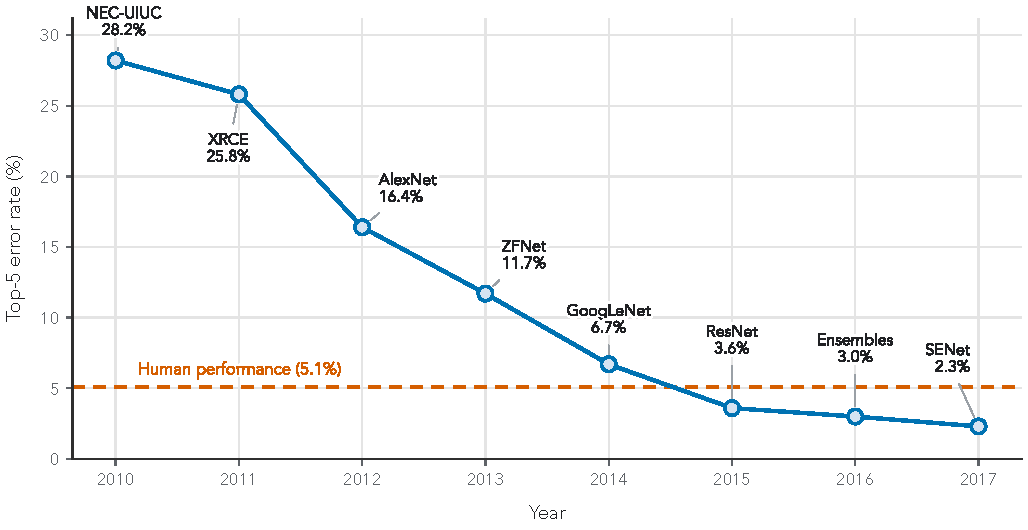
\includegraphics[width=\linewidth]{figures/lit-review/ilsvrc_error_rate_fixed.pdf}
    \caption{ILSVRC Top-5 Error Rate by Year (2010-2017)}
    \label{fig:ch1-ilsvrc-error-rate}
\end{figure}

The confluence of these factors enabled a transition from foundational benchmarking to biologically significant innovation. As performance on general image classification saturated, focus shifted to higher-order tasks, such as object detection, semantic segmentation, and automated feature extraction. These methodologies proved directly applicable to spatial and visual biological data, catalyzing innovation in image-based phenotyping, geospatial modeling, and multimodal artificial intelligence. Consequently, examining the evolution of computer vision is essential to understanding the technological development of modern biological modeling.

\subsection{Origins}\label{sec:ch1-origins}
Much like general deep learning research (Section~\ref{sec:ch1-cybernetics}), computer vision research began as a biologically inspired field grounded in neuroscience principles. In the late 1950s and early 1960s, Hubel and Wiesel provided the theoretical underpinnings for modern architectures with their work on the mammalian visual cortex~\cite{hubel1959receptive, hubel1962receptive}. They showed that vision is a hierarchical process built on detecting and combining local features. The visual cortex does not respond to the retinal input holistically; instead, neurons respond to stimuli within small, specific regions called receptive fields. Additionally, Hubel and Wiesel identified two types of cells involved in processing this visual information: simple cells and complex cells. While simple cells fire only when a specific feature, like a horizontal or vertical line, appears in a precise location, complex cells activate when the feature appears anywhere in the receptive field. Based on these fundamental units, they proposed a hierarchical model of visual processing: simple cells connect to complex cells, which connect to hypercomplex cells, allowing the visual cortex to build a layered representation that abstracts from lines to shapes and eventually to objects.

Kunihiko Fukushima built on this work by introducing the cognitron in 1975 and the neocognitron in 1980~\cite{fukushima1975cognitron, fukushima1980neocognitron}. A precursor to modern CNNs, the neocognitron operationalized the concepts of receptive fields, simple cells, and complex cells from Hubel and Wiesel. Instead of having fully connected layers like the perceptron~\cite{rosenblatt1958perceptron}, the neocognitron featured a shared weight mechanism. This simulated simple cells (referred to as ``S-cells'' by Fukushima) by applying the same filter to each part of the image, meaning a cell would activate any time its filter matched the input pattern in a region. Multiple S-cells could be applied to the image in parallel to detect multiple features. These features were then propagated to complex cells, or C-cells, for transformation-invariant feature detection. S-cells are equivalent to convolution operations, and C-cells are equivalent to pooling operations. The combination of multiple S-C layers resulted in a similar hierarchical structure to the model of visual processing introduced by Hubel and Wiesel~\cite{hubel1959receptive, hubel1962receptive}. Although Fukushima made foundational contributions to CNN architecture, the neocognitron relied on unsupervised competitive learning rather than backpropagation, which hindered its standalone success for complex supervised tasks.

In 1989, Yann LeCun combined the architectural foundations of Fukushima~\cite{fukushima1975cognitron, fukushima1980neocognitron} with the learning rules of Rumelhart et al.~\cite{rumelhart1986learning} to train the first modern CNNs~\cite{lecun1989handwritten}. LeCun used backpropagation to train a CNN for recognizing digits from the United States Postal Service. The model achieved a 1\% error rate and 9\% rejection rate, demonstrating state-of-the-art performance on a real-world task. This result showed that utilizing convolutions for computer vision tasks was a promising approach; because the model learned hierarchical features, the need for manual preprocessing was minimized. Furthermore, the computational burden of these networks was lower than fully-connected networks due to their shared-weight design. Additionally, LeCun argued that the reduction in free parameters caused by the architectural choice reduced overfitting, providing more evidence for the potential of CNNs in computer vision.

LeCun produced multiple iterations on this approach, introducing LeNet-5 in 1998~\cite{lecun1998gradient}. This work expanded the results from LeCun's original paper by scaling the dataset and model size while providing a comparison to other gradient-based models. LeNet-5 achieved performance superior to most existing methods and comparable to Support Vector Machines (SVMs), while offering significantly faster inference speeds. LeCun noted that ``better pattern recognition systems can be built by relying more on automatic learning and less on hand-designed heuristics''~\cite{lecun1998gradient}. The combination of scale and performance in these experiments solidified CNNs as one of the primary methods for image classification. Additionally, the LeNet-5 paper introduced a modular paradigm for neural network programming, introducing various forward and backward propagation functions that could be composed while still storing a computational graph. This framework provided a predecessor to popular deep learning libraries such as Caffe~\cite{caffe}, TensorFlow~\cite{tensorflow2015-whitepaper}, Pytorch~\cite{paszke2019pytorch}, and Jax~\cite{jax2018github}.

Despite CNNs showing successful performance at scale, training was still constrained by hardware and data limitations. LeNet-5 took three days to train for 20 epochs, and the MNIST dataset was still small by modern standards, containing only around 60,000 images. However, as discussed in Section~\ref{sec:ch1-deeplearning}, innovations in these realms promoted more successful computer vision research, with the ILSVRC~\cite{ILSVRC15} serving as the catalyst for rapid progress. 

\subsection{The ImageNet Challenge}\label{sec:ch1-imagenet}
As introduced in Section~\ref{sec:ch1-deeplearning}, the ImageNet dataset~\cite{deng2009imagenet} revolutionized computer vision research, providing a massive, open-source dataset for researchers to benchmark their methods. Due to its popularity, the creators of ImageNet introduced the ILSVRC, which created a standardized benchmark for the deep learning community. As noted earlier, many seminal contributions used the ILSVRC as their primary benchmarking dataset. We will discuss the impact of key ILSVRC participants in this section.  

The first major breakthrough related to the ILSVRC was the introduction of AlexNet~\cite{krizhevsky2012imagenet}, which won the competition in 2012. AlexNet achieved a reduction in top-5 error rate of over 10 percentage points compared to the previous winner, producing ``by far the best results ever reported on these datasets'' at the time~\cite{krizhevsky2012imagenet}. The AlexNet architecture revolutionized deep learning with several contributions. Primarily, the authors were the first to utilize model parallelism with GPUs to train larger models more efficiently. They used two GPUs, partitioning convolutional filters between the two to parallelize processing. Despite being one of the largest CNNs ever at the time, training took a relatively modest five to six days. Furthermore, AlexNet was the first network to utilize dropout~\cite{srivastava2014dropout}, ReLU~\cite{glorot2011deep}, and data augmentation at scale. The adoption of these techniques, combined with the competition-winning performance they yielded, solidified AlexNet as a foundational work and exemplified the superiority of deep learning for image recognition over other techniques, like SVMs, which were popular at the time. It is also important to note that AlexNet's success was a precursor to modern deep learning scaling laws, which will be discussed further in Section~\ref{sec:ch1-llms}; the authors demonstrated that using more compute and data had a direct relationship with performance, a trend that continued to be explored in the following years across various deep learning subdomains.

In 2014, two innovative architectures achieved first and second place in the ILSVRC. GoogLeNet~\cite{szegedy2015going}, developed by researchers at Google, won the competition, while VGGNet took second place. GoogLeNet utilized an architecture called ``Inception,'' which enabled the training of even deeper CNNs while using fewer parameters. Each inception block balanced receptive field focus by using 1 $\times$ 1, 3 $\times$ 3, and 5 $\times$ 5 convolutional kernels in parallel in a single layer; the varied kernel sizes created an implicit balance between hierarchy and localization. Crucially, to reduce the number of parameters in the network, and thus overfitting, GoogLeNet utilized global average pooling to transform the inception outputs for classification rather than the dense layers used in prior work. Due to the shared weights of convolutions, this greatly reduced the parameter burden compared to using fully-connected layers, which previous architectures like AlexNet had relied on for reshaping outputs~\cite{krizhevsky2012imagenet}. Finally, GoogLeNet leveraged auxiliary classification to increase network depth. The authors added outputs at intermediate layers in the network; by performing backpropagation from these auxiliary objectives, they ensured a strong gradient signal throughout the network, even with increasing depth. The combination of these innovations produced the most performant model of the time.

While GoogLeNet's Inception architecture showed that a complex, highly engineered CNN could yield state-of-the-art performance, VGGNet took an alternate approach, demonstrating that a homogeneous network with many layers of small convolutions could yield comparable performance~\cite{simonyan2014very}. The authors tested CNNs of various depth while exclusively using 3 $\times$ 3 convolutional filters, arguing that stacks of smaller filters were equivalent to a single, larger filter while fitting a more discriminative function with fewer parameters. They demonstrated this result empirically, achieving second place in the ILSVRC and first place in the ImageNet localization competition. This homogeneous, stacked architecture provided an easily scalable structure, and its simplicity led to its adoption across multiple other subdomains.

In 2015, superhuman performance was formally achieved in the ILSVRC with the introduction of ResNet~\cite{he2016deep}. The primary focus of the ResNet architecture was combating the vanishing gradient problem, which, despite being partially addressed by innovations such as ReLU~\cite{glorot2011deep}, was still prevalent as network depth exceeded 30 layers. The ResNet team introduced residual learning, where instead of fitting a function, $h(x)$, its residual, $h(x)-x = f(x)$, was learned. Consequently, layer mappings could be reformulated as learning $f(x)+x$, including a direct connection from the input to the output of a layer. This directly addressed gradient saturation by providing a residual stream without exposure to a nonlinearity, stabilizing gradient flow. By adding residual connections to an architecture inspired by VGGNet, the authors were able to train networks with a depth of up to 152 layers. The innovations introduced in ResNet have been adopted by numerous state-of-the-art architectures across subdomains, showing the impact of this work.

Over its life cycle from a difficult, open research competition to a saturated benchmark, the ILSVRC yielded many innovative approaches to image classification. Model parallelism~\cite{krizhevsky2009learning}, dropout~\cite{srivastava2014dropout}, ReLU~\cite{glorot2011deep}, homogeneous block architectures~\cite{simonyan2014very}, and residual connections~\cite{he2016deep} are all used in various architectures across subdomains today. In the next section, we will discuss how these methods were incorporated to address the challenges of semantic segmentation and object detection.

\subsection{Semantic Segmentation}\label{sec:ch1-segmentation}

As performance on the ILSVRC improved, the benchmark became saturated; state-of-the-art models reached an accuracy plateau where meaningful improvements became diminishingly marginal. Due to this saturation, focus shifted to more complex tasks such as semantic segmentation, where specificity and localization carried greater weight. In biology, semantic segmentation is critical; for example, pixel-level classification enables researchers to extract intensive phenotypes from images, facilitating population-scale studies. Therefore, it is important to understand advances in semantic segmentation to understand how best to apply it to biological data.

While semantic segmentation was historically strongly tied to the ImageNet dataset, one of the first state-of-the-art segmentation models was developed for biomedical image segmentation. U-Net~\cite{ronneberger2015u}, developed in 2015, is a fully convolutional architecture that produces pixel level classifications to create image segmentation maps. The architecture features a contractive path to capture hierarchical and contextual features followed by a symmetric expansive path to provide specific localizations within the image. The contractive and expansive paths are also linked via skip connections. Functionally similar to residual connections~\cite{he2016deep}, skip connections improve gradient flow in the model while also enabling the combination of hierarchical features with localized features via concatenation in the expansive feature map~\cite{ronneberger2015u}. U-Net achieved state-of-the-art performance on both \textit{Drosophila} nerve membrane segmentation and cellular segmentation, solidifying its role as a biologically useful deep learning architecture.

Despite the success of U-Net, its supervised nature meant that ground-truth pixel-level segmentation data was necessary for training. Such data is expensive and tedious to collect, so naturally, researchers began to explore other architectures to reduce the burden of collecting hand-labeled segmentations. One of the first attempts to explore deep, unsupervised image segmentation was W-Net~\cite{xia2017wnet}. This architecture combined two U-Nets to produce a segmentation map without supervision. The first U-Net produced a \textit{k}-channel representation of the image, with \textit{k} representing the number of classes for segmentation. This segmentation map was then propagated through another U-Net, which reconstructed the input. The intermediate segmentation map was evaluated with a soft normalized cut loss function, which maximizes association between pixel groups, while the final reconstruction was evaluated with a reconstruction loss function. By jointly optimizing these two functions, the W-Net architecture could extract segmentations in an unsupervised manner. After training, conditional random field smoothing was applied to improve segmentation quality. W-Net produced results comparable to the state-of-the-art unsupervised segmentation models, providing an alternative to the labor-intensive process required to produce datasets for supervised semantic segmentation. 


In 2017, He et al. introduced Mask R-CNN, an alternative architecture that unified object detection, instance segmentation, and classification into a multi-task objective~\cite{he2017mask}. Expanding on the work of the Fast R-CNN~\cite{girshick2015fast} and Faster R-CNN~\cite{ren2016faster}, which explored only classification and object detection, the Mask R-CNN added a semantic segmentation path that was trained simultaneously with the classification and bounding box objectives. Unlike semantic segmentation, which labels all pixels of a class identically, this approach enabled instance segmentation, distinguishing between individual objects of the same class. This architecture achieved state-of-the-art performance on the common objects in context (COCO) dataset~\cite{lin2014microsoft} and human pose estimation, showing the transferability and generality of the Mask R-CNN method.

Despite the success of Mask R-CNN and U-Net, the explosive success of transformer architectures in the language modeling domain (detailed in section~\ref{sec:ch1-llms}) inspired novel approaches to computer vision. Dosovitskiy et al. introduced the vision transformer (ViT) in 2020~\cite{dosovitskiy2020image}; instead of relying on convolutional layers, which were the standard for computer vision architectures, the authors leveraged the attention mechanism. By dividing images into 16 $\times$ 16 pixel ``patches,'' and encoding these patches into tokens with a linear layer, the ViT architecture allowed images to be processed as sequences. This solution addressed many concerns in the original W-Net paper regarding data efficiency; while the original ViT was supervised, it established the architectural framework that later enabled powerful self-supervised masked imaged modeling (such as MAE), reducing reliance on expensive labeled data~\cite{xia2017wnet}. Although not strictly a segmentation model, the ViT created a framework that enabled transformer-powered segmentation.

Building on the ideas introduced by the ViT, researchers at Meta released the Segment Anything Model (SAM) for semantic and instance segmentation~\cite{kirillov2023segment}. SAM is a foundation model built with a ViT architecture, trained on over 11 million images and 1 billion segmentation masks with a model-in-the-loop paradigm. Newer versions, SAM 2~\cite{ravi2024sam} and SAM 3~\cite{carion2025sam3} were released in 2024 and 2025, respectively, to enable video segmentation, improve inference speed, and enhance text prompting.

\subsection{Transformer-Based Segmentation}\label{sec:ch1-tfseg}

\section{Language Modeling}\label{sec:ch1-llms}
Like computer vision, language modeling has been a proving ground for deep learning, with the two subdomains evolving in parallel. As in other deep learning domains, language modeling and the architectures stemming from it are shaped by the properties of data through inductive biases. Modeling language assumes sequentiality, contextual dependence, and variable length. Sequentiality is the assumption that the order of words in a sentence matters; changing a sentence's order implies changing its meaning. Contextual dependence is the assumption that the meaning of a word changes depending on the words around it. Variable length is the assumption that sentences can be of arbitrary length, meaning that models must be designed to handle heterogeneity in sequence length. These assumptions are critical to understanding the evolution of language modeling and the architectures that have been developed to address them. Additionally, like computer vision, language modeling comprises various tasks that are related. Examples include next-token prediction of a discrete vocabulary for language generation, masked token prediction for representation learning and classification, and sequence-to-sequence modeling for translation. Critically, many of these objectives are self-supervised,  These tasks are often interrelated, with advances in one task often informing the development of others.

In this section, we will discuss the evolution of language modeling, beginning with the origins of the field in Section~\ref{sec:ch1-lm-pretransformer}, followed by the introduction of the transformer architecture in Section~\ref{sec:ch1-transformer}. We will conclude with the reinforcement learning methods used to steer model behavior after pre-training in Section~\ref{sec:ch1-rl}.

\subsection{From Counting to Recurrence}\label{sec:ch1-lm-pretransformer}
The statistical treatment of language was formalized by Claude Shannon in 1948. Shannon formulated text as a stochastic process, establishing natural language as having a measurable statistical structure; this structure could be exploited to predict the next word in a sequence, which is the fundamental objective of language modeling~\cite{shannon1948mathematical}. 
Specifically, modeling the probability of a sequence of words occuring, $P(A,B,C)$, can be decomposed into a product of conditional probabilities:
\begin{equation}
    P(A,B,C) = P(A)P(B|A)P(C|A,B).
\end{equation}
Early language models were based on this principle, applying a Markov assumption of order $n-1$ to predict the next word from the previous $n-1$ words~\cite{chen1999empirical}. However, these models, called \textit{n-gram} models, were limited by the curse of dimensionality~\cite{bengio2003neural}; as $n$ increased, the number of possible sequences grew exponentially, making it impossible to estimate probabilities for all sequences. For example, modeling 10 consecutive words with a vocabulary of 100,000 words would require estimating $100{,}000^{10} = 10^{50}$ probabilities, which is infeasible~\cite{bengio2003neural}. Therefore, n-gram models were limited to small values of $n$, typically bigrams or trigrams~\cite{chen1999empirical}.

However, n-gram models were still subject to another failure case: if a sequence of words was not observed in the training data, the model would assign it a probability of zero, a failure that drives cross-entropy to infinity~\cite{chen1999empirical}. This motivated the development of smoothing techniques, which redistributed probability mass to unseen sequences~\cite{chen1999empirical}. Despite the modeling improvements that these techniques yielded, their ultimate failure was limited by the representation of words as discrete. By modeling words as discrete tokens, n-gram models could not capture semantic relationships between words, such as synonyms or antonyms~\cite{bengio2003neural}. This limitation motivated the development of learning distributed representations for words, catalyzing research in neural language modeling.

Distributed representations, known today as word embeddings, were first introduced by Bengio et al. in 2003~\cite{bengio2003neural}. Recognizing the difficulty of discrete language modeling, Bengio et al. proposed a neural architecture that learned a continuous vector representation of words, allowing the model to capture semantic relationships between them. The initial layer in the architecture was a lookup table that mapped each token in the vocabulary to a continuous vector, allowing the discrete representation to be distributed continuously in vector space. This theoretical framework, combined with the empirical success demonstrated in the work, motivated word embedding as a standard component of modern language modeling. 

Building on Bengio et al.'s work, Mikolov et al. introduced the word2vec framework in 2013~\cite{mikolov2013efficient}. Word2vec is neural language architecture that learns word embeddings by predicting the context of a word in a sentence. Training on a significantly larger corpus than previous work, the authors demonstrated that the learned embeddings from their model captured semantic relationships between words, such as synonyms and antonyms. This allowed vector operations to be performed on the embeddings, enabling analogical reasoning. For example, the vector operation $v(\text{king}) - v(\text{man}) + v(\text{woman})$ produces a vector that is closest to $v(\text{queen})$, demonstrating that the model learned the relationship between gendered words. This work was a major breakthrough in language modeling, demonstrating that neural architectures could learn meaningful representations of words from large corpora of text.

However, the conceptual breakthroughs in language modeling required architectural innovation to be brought to fruition. The first widely-used neural architecture for language modeling was the recurrent neural network (RNN), introduced by Jeffery Elman in 1990. The RNN consists of a hidden state, $h_t$, that is updated at each time step based on the current input, $x_t$, and the previous hidden state, $h_{t-1}$. This structure allows the network to maintain a memory of previous inputs, enabling it to model sequential data~\cite{elman1990finding}. 

While RNNs imbued neural networks with a memory mechanism, their context length was limited by the vanishing gradient problem. As sequences grew longer, the gradient signal that propagated through the RNN's hidden states would either vanish or explode, making training on long sequences unstable. To address this shortcoming, Hochreiter and Schmidhuber introduced the long short-term memory (LSTM) architecture in 1997~\cite{hochreiter1997long}. The LSTM introduced a cell state, $c_t$, in addition to the hidden state. The cell state is updated at each time step based on the current input, using a series of gates the control the flow of information. Because the cell state is updated without nonlinearities, the gradient signal can propagate through the network without vanishing or exploding, allowing the LSTM to maintain a memory of previous inputs over long sequences and making them the dominant architecture for language modeling for nearly two decades. 

Neural language modeling began its domainance of statistical language modeling in 2014, when Sutskever et al. employed LSTMs to achieve state-of-the-art performance on machine translation~\cite{sutskever2014sequence}. Sutskever et al. used two LSTMs: and encoder to represent the source sequence, and a decoder to generate the target sequence. The encoder's hidden state, which contained a representation of the source sequence, was used to initialize the decoder's hidden state, transferring information from the source to the target. This architecture, called sequence-to-sequence (seq2seq), was a major breakthrough in neural language modeling, demonstrating that LSTMs could be used to model complex sequential data and achieve state-of-the-art performance on machine translation tasks.

Less that a year later, Bahdanau et al. introduced the attention mechanism to improve the seq2seq architecture~\cite{bahdanau2014neural}. Bahdanau et al. argued that the seq2seq architecture was limited by the fixed-length representation of the source sequence, which was a bottleneck for long sequences. Instead, they proposed an attention mechanism that allowed the decoder to compare its current state to the encoder's hidden states and gather information from the most relevant parts of the source sequence. The introduction of attention laid the foundation for the transformer architecture, which would revolutionize language modeling.

\subsection{Transformer}\label{sec:ch1-transformer}
The transformer architecture was introduced by Vaswani et al. in 2017~\cite{vaswani2017attention}, with the original work once again being applied to machine translation. The transformer architecture is based on the attention mechanism, which allows the model to weight the importance of different parts of the input sequence when generating an output. The original transformer architecture consisted of an encoder and decoder, each composed of multiple transformer blocks that featured multi-head self-attention and feedforward layers. As in seq2seq, the encoder generates a representation of the input sequence, which is then used by the decoder to generate the output sequence. Because self-attention is permutation-invariant, positional information must be injected explicitly; the original work added sinusoidal positional encodings to the input embeddings~\cite{vaswani2017attention}. However, the attention mechanism allows the transformer to excel at capturing long-range dependencies, and the model's lack of a hidden state makes it parallelizable on the time dimension. These properties allow the transformer to scale to larger datasets and model longer sequences than previous architectures, making it a powerful tool for language modeling.

Building on the success of the transformer architecture, OpenAI introduced the Generative Pre-trained Transformer (GPT) in 2018~\cite{radford2018improving}. Notably, the GPT models are decoder-only architectures; instead of producing a target sequence from an input sequence, they predict the next token in a sequence given previous tokens - the same modeling approach as n-gram models. The original model, GPT-1~\cite{radford2018improving}, was pre-trained on a large corpus of text using a negative log-likelihood objective, and then fine-tuned on specific tasks using labeled data. This pre-training and fine-tuning paradigm allowed the model to learn general language representations that could be adapted to specific tasks while achieving state-of-the-art performance.

Extending the GPT-1 architecture, OpenAI released GPT-2 in 2019~\cite{gpt2}. While GPT-1 was fine-tuned on specific tasks after pre-training, GPT-2 demonstrated that the model could achieve state-of-the-art performance on several tasks without fine-tuning, using only prompted examples during inference time. This zero-shot learning capability demonstrated that models could show emergent behavior when scaled to larger sizes, generalizing to tasks outside of their training corpus. Additionally, the release of GPT-2 began to popularize foundation modeling, where a single model is pre-trained on a large corpus of data and then adapted to specific tasks. 

Building on the emergence through scaling that was observed in GPT-2, OpenAI released GPT-3 in 2020~\cite{brown2020language}. GPT-3 was scaled to 175 billion parameters, two orders of magnitude larger than GPT-2, and trained on more text data. Additionally, the concept of in-context few-shot learning was introduced; rather than fine-tuning the model on a specific task, merely supplying a few examples of the task during prompting was sufficient to achieve state-of-the-art performance. This phenomenon demonstrated that large language models could generalize to new tasks without task-specific training, further solidifying the foundation modeling paradigm.

In addition to the success of autoregressive language modeling, the transformer architecture had been applied to a variety of other tasks. BERT~\cite{bert} uses a masked language modeling objective to learn representations of text, ViT~\cite{dosovitskiy2020image} uses a transformer architecture to process images, and CLIP~\cite{radford2021learning} uses a transformer architecture to learn joint representations of images and text. These models have achieved state-of-the-art performance on a variety of tasks, demonstrating the versatility and power of the transformer architecture.

Furthermore, several architectural innovations have been made to improve the efficiency and scalability of transformer models. Most notably, the feed-forward blocks in modern transformers are often replaced with sparse mixture-of-experts (MoE) layers~\cite{shazeer2017outrageously} which allow more parameters to be used without increasing the computational cost of inference. Context extension techniques such as YaRN~\cite{peng2023yarn} and RoPE~\cite{su2024roformer} have allowed models to better handle massive contexts, and parameter-efficient fine-tuning (PEFT) methods such as low-rank adaptation (LoRA)~\cite{hu2022lora} allow models to be adapted to new tasks without retraining every parameter.

\subsection{Reinforcement Learning and Post-Training}\label{sec:ch1-rl}
While transformer models trained for next token prediction demonstrated strong performance on a variety of tasks, they were not without limitations. Although pre-training imbues the model with the \textit{capability} to generalize to many tasks, it does not guarantee the model's \textit{behavior}. In many cases, labeled datasets do not exist to train the model's behavior through imitation learning, so reinforcement learning (RL) is used instead to steer the model's behavior through comparative judgements and verifiable rewards. However, a core challenge of RL is credit assignment; in the case of language model post-training, how does one determine which tokens in a sequence were responsible for correct or incorrect outomes? Even if one can identify the relevant tokens, assigning credit to them through backpropagation is non-trivial. To address these challenges, it is important to examine the lineage of RL methods that have been developed to train large language models.

RL was formalized in 1984 by Richard Sutton~\cite{Sutton84}, who defined the process as a Markov decision process (MDP) with an agent, environment, state, and reward. The agent takes actions in the environment, transitioning between states and receiving rewards based on its actions. The goal of the agent is to learn a policy that maximizes the expected cumulative reward over time. Sutton's work laid the foundation for RL research, which has since been applied to a variety of domains. 

Sutton's work was extended to language modeling with the introduction of trust region policy optimization (TRPO)~\cite{schulman2015trust}. TRPO is a policy gradient method which constrains the policy update to a trust region with Kullback-Leibler (KL) divergence, ensuring that the new policy is not too far from the old policy. However, TRPO is complex to implement and requires second-order optimization, which can be computationally expensive.

Building on TRPO, proximal policy optimization (PPO) was introduced in 2017~\cite{schulman2017proximal}. Proximial policy introduced a clipped importance ratio to constrain the policy update, simplifying the optimization process while improving performance. PPO's clipped objective ensures that a single update does not change the policy too much in the direction of positive-reward actions, while still allowing the penalty to for negative-reward actions to be unbounded. PPO has become a standard method for RL in language modeling.

Additionally in 2017, reinforcement learning with human feedback (RLHF) was introduced by Christiano et al.~\cite{christiano2017rlhf}. Rather than relying on numerical rewards, which can be difficult to define in many tasks, RLHF uses human preferences to train a reward model that guides the agent's behavior. The reward model is trained on a dataset of human-labeled comparisons between different outputs, allowing the agent to learn a policy that aligns with human preferences. 

In 2022, OpenAI unified PPO and RLHF into a single framework for training large language models with the release of InstructGPT~\cite{ouyang2022instructgpt}. Language, like many other domains, is difficult to quantify; therefore, InstructGPT used human feedback to train a reward model. The authors replaced the numerical reward function in PPO with a learned reward model to optimize InstructGPT with policy gradient methods, yielding a model that was well aligned with human preferences despite only being trained with human preference comparisons. This result set a new standard for large language model training.

However, several limitations of RLHF prompted new methods to be explored. RLHF can be unstable, requiring careful tuning of the reward model and the policy during training. Additionally, RLHF is computationally expensive due to the dual optimization that takes place. Therefore, direct preference optimization (DPO)~\cite{dpo} as an alternative method for preference alignment. DPO reformulates the RLHF objective as an offline objective, where the model is directly optimized against recorded human preference comparisons. This approach simplifies the optimization process and reduces the computational cost of training, while still achieving strong performance on preference alignment tasks.

We the above methods all address preference alignment within language models, other approaches have been introduced for reinforcement learning through verifiable rewards. Verifiable domains, such as coding, math, and logic, have clear correctness criteria that can be used to update the model's policy. DeepSeekMath~\cite{shao2024deepseekmath} introduced group-relative policy optimization (GRPO). Due to cheap, calculable rewards in the domain of mathematics, GRPO samples from a group of rollouts and calculates the advantage as the divergence of a rollout from the group mean. This approach also reduces the trainable parameters compared to PPO by roughly one half, since a value model is not required. 

DeepSeek built on the GRPO framework by releasing DeepSeek-R1\cite{guo2025deepseek}, which post-trained a large language using GRPO. The authors demonstrated that a model post-trained solely with RL could achieve competitive performance with models that included an SFT stage, and they observed emergent behaviors like backtracking and self-correction. This result suggests that RL is an essential component of model post-training to induce reasoning behavior via rewards.

\section{High-Performance Computing for Deep Learning}\label{sec:ch1-hpc}
High performance computing (HPC) has been a critical enabler of deep learning research and its commercial success. As the centers of innovation have shifted from academia to industry, the scale of research has expanded, and with it the computational resources required to train state-of-the-art models. In this section, we will discuss the scaling laws that motivated HPC use for deep learning, and then discuss the HPC strategies that are employed to train large models across multiple GPUs and nodes.

\subsection{Scaling Laws}\label{sec:ch1-scaling}
A central theme in deep learning is that larger models trained on more data with more compute tend to perform better. This was seen in the ImageNet competition, where AlexNet~\cite{krizhevsky2012imagenet} used a very deep architecture to achieve state-of-the-art performance, an in language modeling, where GPT-3~\cite{brown2020language} demonstrated that scaling to 175 billion parameters yielded emergent capabilities. However, for most of the history of deep learning, this relationship was anecdotal. 

In 2020, Kaplan et al. formalized the relationship between model size, dataset size, and compute budget in a series of scaling laws~\cite{kaplan2020scaling}. The authors first demonstrated that scaling is architecture insensitive, implying that these laws are generalizable across deep learning subdomains. They also demonstrated the relationship that each of these three factors has with performance, showing that model loss decreases in a power law relationship with increasing model size, dataset size, and compute budget. This relationship, along with the finding that small-scale experiments can forecast large-scale results, was a motivating factor for the development of large language models, which today can be trained trillions of parameters on trillions of tokens.

However, some details in the original scaling laws were corrected with the release of Chinchilla~\cite{hoffmann2022training}. While Kaplan et al. implied that model size should grow faster than dataset size, Hoffmann et al. showed that most models were badly undertrained, and parameters and tokens should scale at a 1:1 ratio. While this result didn't challenge the notion that larger models trained on more data with more compute perform better, it did frame a concrete question for future work: given a fixed FLOPs budget, how should one trade off model size against training tokens?

The observation of these concrete scaling laws has motivated the development larger and larger models. However, as model size increases, it no longer becomes feasible to train models on a single GPU, or even a single node. Therefore, the remainder of this section will discuss the distributed training strategies that have been developed to enable the training of large models at the billion- and trillion-parameter scale.

\subsection{Distributed Training Strategies}\label{sec:ch1-distributed}
A variety of distributed training strategies have been developed to meet the scaling needs of deep learning, which can be compute-bound in many ways. Data parallelism is a common strategy for improving model throughput; specifically, distributed data parallelism (DDP)~\cite{li2020pytorch} replicates the model weights across multiple GPUs, and each GPU is responsible for computing the forward and backward passes on a subset of the training data. After each GPU computes its gradients, they are all-reduced to synchronize model weights. This approach is effective for models that fit within a single GPU's memory, but as model size increases, it becomes infeasible to replicate the model across multiple accelerators.

Therefore, the rest of this section covers model parallelism, which divides that model across multiple GPUs to enable training of models that are memory-bound. In order to shard a model across accelerators, different states must be partitioned across GPUs. DeepSpeed ZeRO and fully-sharded data parallelism (FSDP)~\cite{rajbhandari2020zero, zhao2023fsdp} are two popular approaches for handling model states. DeepSpeed ZeRO partitions the optimizer states, gradients, and parameters of a model across GPUs in separate stages: Zero-1 partitions only optimizer states, ZeRO-2 partitions optimizer states and gradients, and ZeRO-3 partitions optimizer states, gradients, and parameters. FSDP partitions all model states across GPUs, but uses a pytorch-specific implementation.

In addition to sharded model parallelism, tensor parallelism~\cite{shoeybi2019megatron} is a strategy for partitioning the computation of a single layer across devices, separating row- and column-wise operations for different parts of the layer. Pipeline parallelism~\cite{huang2019gpipe} shards different layers of the model across devices, allowing for concurrent execution of different layers on different GPUs. Expert parallelism~\cite{lepikhin2020gshard} moves different experts in an MoE layer to different GPUs, and context/sequence parallelism~\cite{jacobs2023ulysses} divides the input sequence across GPUs, allowing for longer contexts to be processed. These strategies can be combined into multi-dimensional parallelism~\cite{narayanan2021efficient}, which allows for the training of models with trillions of parameters on thousands of GPUs. Overall, the combination of these distributed training strategies has enabled the scaling of large language models to sizes that were previously infeasible, allowing for the exploration of emergent behaviors and capabilities.

\section{Deep Learning for Biology}\label{sec:ch1-biology}
While deep learning has achieved notable success in domains such as computer vision and natural language processing, its application to biological data remains comparatively less mature. Unlike image or text modalities, biological data exhibit complexity, hierarchical structure, and long-range dependencies, all with limited or noisy supervision. These characteristics challenge many of the assumptions that underlie standard deep learning architectures and training paradigms. As a result, biological problems provide compelling settings to test how advances in representation learning, model scaling, and computational infrastructure generalize beyond areas where deep learning has been most successful. Understanding of prior work in vision, language modeling, and scalable training is therefore essential for situating and motivating the approaches explored in this proposal.

\subsection{Vision-Based Phenotyping}

\subsection{Deep-Learning Based Genomic Prediction}\label{sec:ch1-genomicpred}
To understand the potential benefits of deep learning for genomic prediction and selection, it is crucial to understand the foundations and current state of the field. Traditionally, genomic prediction has relied on statistical models to estimate breeding values from genotypic data. Meuwissen et al. introduced genomic selection~\cite{meuwissen2001prediction}, fitting linear models with shrinkage to dense single nucleotide polymorphism (SNP) marker data to predict breeding values. VanRaden later formalized the genomic best linear unbiased predictor (GBLUP) by deriving a genomic relationship matrix from marker data and substituting it for the pedigree relationship matrix in the mixed model equations~\cite{vanraden2008efficient}, improving predictive accuracy. However, these methods are limited by their linear assumptions and inability to capture complex interactions between genetic variants.

Jarquin et al. introduced the reaction norm model~\cite{jarquin2014reaction} in 2014, which extended the GBLUP framework to account for genotype-by-environment (G$\times$E) interactions using genomic, environment, and G$\times$E kernels. This model improved predictive accuracy in multi-environment trials, but the interaction structure still had to be specified a priori through the choice of kernel.

Therefore, deep learning methods have provided a contrasting approach to modeling genomic data. Due to the complex nonlinear relationships between genetic variants, environmental variables, and phenotypic traits, deep learning methods may excel in genomic prediction tasks. Early deep learning methods for genomic prediction used MLPs and CNNs for prediction, such as Bellot et al.~\cite{bellot2018can} and Khaki and Wang~\cite{khaki2019crop}. However, these methods have yet to consistently outperform linear models~\cite{montesinos2021review, azodi2019benchmarking}. Researchers speculate that linear models such as GBLUP are already well matched to the largely additive genetic architecture of many traits, leaving deep learning models with few opportunities to improve performance. Additionally, marker inputs are structurally impoverished, typically encoded as allele dosages at each locus, offering little for a deep model to exploit beyond the additive signal a linear model already captures. Recent work, however, has shown that shaping the inductive biases of deep learning models to better reflect the underlying biology can improve performance.

Inspired by the success of sequence models for language modeling, several recent works have applied transformer architectures to genomic modeling. Broadly, these works fall into two categories: reference-sequence foundation models and genotype-matrix models over individuals. Reference-sequence foundation models pretrain on genomic sequences, learning general representations of genomic data, and are then evaluated on functional or regulatory tasks. DNABERT~\cite{dnabert} and DNABERT-2~\cite{dnabert2} each trained a bidirectional transformer to learn genomic sequence representations through masked language modeling. The Nucleotide Transformer~\cite{nucleotide-transformer} scaled this approach across human and multi-species genomes, and Caduceus~\cite{caduceus} replaced attention with a bidirectional state-space backbone that respects reverse-complement symmetry, extending the sequence context these models can process. Because they are pretrained on reference genomes and evaluated on functional and regulatory tasks, however, these models learn general sequence representations rather than predicting phenotypes across a population of individuals.

The second category consists of genotype-matrix models, which operate over the variant genotypes of many individuals and therefore align more directly with the genomic prediction task. SNP2Vec~\cite{snp2vec} adapted subword tokenization to diploid variant sequences, pretraining representations of genomic variation for downstream association tasks, while SNVformer~\cite{snvformer} applied an efficient attention variant to single nucleotide variant data, treating association analysis as a supervised sequence problem rather than a series of independent univariate regressions. GPformer~\cite{wu2023transformer} embedded markers with a convolutional block before a transformer encoder and regression head, coupling the architecture with a knowledge-guided module to predict quantitative phenotypes. Most relevant to this proposal, GEFormer~\cite{geformer} targeted G$\times$E prediction directly, encoding markers with a gated multilayer perceptron and daily environmental measurements with dynamic convolution and linear attention, then combining the two representations through a gating mechanism. This branch-based design is characteristic of multimodal genomic prediction models, in which marker--environment interactions can form only after each modality has been encoded independently.

In recent years, several efforts have standardized genomic prediction and selection research under unified benchmarks. Notably, in the plant research community, the Genomes to Fields (G2F) Maize Prediction Competition~\cite{g2f-2024-competition} has provided a benchmark for evaluating G$\times$E prediction methods, including deep learning approaches. This large, multi-modal dataset and competition structure provide a testbed that is analogous to the role of the ILSVRC in computer vision (Section~\ref{sec:ch1-imagenet}). However, unlike the ILSVRC, the G2F competition has not yet produced a breakthrough result. In Chapter~\ref{ch3:gxe}, we will discuss our efforts using deep learning for G$\times$E prediction on this dataset.

\subsection{LLM-Based Mechanistic Exploration}\label{sec:ch1-llmmech}
Mechanistic interpretation is the process of explaining how biological function arises from the interactions among molecular entities, rather than cataloging those entities individually~\cite{hartwell1999molecular, barabasi2004network}. The object of interpretation is therefore not a single sequence or measurement, but the \textit{interactome}: the set of physical, regulatory, and functional relationships that connect genes, proteins, and metabolites across an organism. These relationships are naturally represented as networks, and the networks themselves are hierarchically structured. Individual interactions aggregate into functional modules, modules participate in pathways, and pathways combine into the higher-order processes that produce a phenotype~\cite{barabasi2011network, menche2015uncovering}. Interpretation operates across these scales simultaneously, since the meaning of a single edge depends on the module and pathway context in which it sits~\cite{ideker2012differential}. Machine learning methods such as iterative random forest~\cite{basu2018iterative, cliff2019high} have expanded the scale and resolution of these networks considerably, but the resulting structures are far larger than any researcher can examine exhaustively, which motivates computational approaches to interpretation itself.

One line of work applies language modeling directly to biological sequence data. Because biological sequences are discrete, ordered, and highly structured, they can be treated as a language and modeled with the techniques described in Section~\ref{sec:ch1-llms}. scGPT~\cite{cui2024scgpt} pretrained a generative transformer over single-cell expression profiles, and protein language models learned representations that support structure and function prediction~\cite{esm3}. We described an analogous line of work for DNA sequence models in Section~\ref{sec:ch1-genomicpred}. These models encode biological knowledge implicitly in their weights, which makes them capable representation learners but poor interpreters; a model that represents a protein cannot traverse the interactome, consult a curated database, or attribute a claim to a source.

Before a language model can reason over a network, it must be able to represent graph structure at all. Evidence that transformers can internalize structured state comes from OthelloGPT~\cite{othellogpt}, in which a model trained only to predict legal moves in a board game developed an internal representation of the board, despite never observing one directly. This result suggests that supervised training on sequences generated by a structured process can induce a representation of the underlying structure. For graphs specifically, Fatemi et al.~\cite{fatemi2024talk} showed that language model performance on graph reasoning tasks depends substantially on how the graph is serialized into text, and that the encoding choice can matter as much as model scale. Together, these results motivate a supervised fine-tuning stage in which a model learns graph rules and operations directly from serialized structure, before any agentic training begins.

Reasoning over that structure requires more than a single forward pass. Chain-of-thought prompting~\cite{wei2022chain} showed that eliciting intermediate reasoning steps substantially improves performance on multi-step problems, establishing that useful computation can be externalized into the token sequence. Tree-of-thoughts~\cite{yao2023tree} generalized this from a single linear trace to a search over a tree of candidate thoughts, with explicit branching, evaluation, and backtracking. This formulation is directly relevant to network exploration, where several starting points may be plausible and unproductive branches should be abandoned rather than followed to completion. ReAct~\cite{yao2022react} extended reasoning traces to include actions, allowing a model to query external sources and condition subsequent reasoning on what it retrieved, while Toolformer~\cite{schick2023toolformer} demonstrated that models could learn when to invoke external tools in a self-supervised manner. Such policies are trained with the post-training methods described in Section~\ref{sec:ch1-rl}. This framing is well suited to mechanistic interpretation because hallucination is disqualifying in this setting; an invented interaction between two genes is not a degraded answer, but a false one.

Several challenges remain when these methods are applied to biological networks. Networks are far too large to fit within a model's context window, so exploration must proceed iteratively rather than in a single pass, and the model must decide what to examine at each step. Mechanistic reasoning is multi-hop, so errors compound across a trajectory, and an incorrect early retrieval can misdirect every step that follows. Unlike mathematics and code, where correctness is cheaply verifiable, there is no ground truth for a correct mechanistic narrative, so reward must be constructed from structural properties of the exploration rather than from a single correct answer. Finally, frontier model inference cost scales with exploration length and reasoning depth, so the most capable models are the least practical for the long-horizon traversal this task demands.

These constraints also shape how the graph should reach the model. One approach encodes graph structure with a learned graph neural network and injects the resulting representation into the model's context~\cite{g-retriever}. Applied to biological networks, this approach faces two practical obstacles. First, it requires trainable graph data, which is considerably harder to obtain than text; curated interaction data is expensive to produce and covers only a small fraction of the interactome. Second, graph neural networks~\cite{kipf2016semi, velivckovic2017graph} are difficult to scale relative to transformers, because neighborhood aggregation is irregular and does not admit the dense, uniform parallelism that the training strategies in Section~\ref{sec:ch1-distributed} depend on. A learned graph encoder also compresses structure into a representation that cannot be traced, which is a liability when the output is a mechanistic claim.

An alternative is a staged approach that keeps the graph external to the model. Supervised fine-tuning first teaches the model general graph structure and operations, unifying graph representation with language space so that the model's reasoning about the network remains expressible in text, and therefore interpretable. Reinforcement learning methods such as DPO~\cite{dpo} and GRPO~\cite{shao2024deepseekmath} then post-train the model on reasoning and exploration tasks, where the branching search described above becomes a learned behavior rather than a prompting strategy. Throughout, the graph is reached through deterministic operators such as neighborhood retrieval, shortest-path search, and random walk with restart~\cite{kainer2025rwrtoolkit}, each of which returns provenance alongside its result, so a claim can be traced back to the graph evidence that produced it.

Recent systems have begun to address these challenges. eubiota~\cite{eubiota} and \textsc{Mentor-IA}~\cite{mentor-ia} demonstrated that provenance-preserving retrieval and tool-mediated synthesis can produce high-fidelity mechanistic narratives over biological networks, building on module structures derived from methods such as \textsc{Mentor}~\cite{mentor}. However, both systems depend on frontier model inference, which limits deployment at the exploration depths that large networks demand, and neither is optimized as a trainable policy. In Chapter~\ref{ch4:mentor-rl}, we will discuss our efforts to train an open-source reasoning agent for mechanistic exploration of biological networks with reinforcement learning.
